

\documentclass[a4paper, 12pt, notitlepage]{report}
\usepackage[T1]{fontenc}
\usepackage{textcomp}
\usepackage{xfrac}

\usepackage[utf8]{inputenc}
\usepackage[english,italian]{babel}
\usepackage{verbatim}
\usepackage{listings}

\usepackage{hyperref}
\usepackage{etoc}

\usepackage{float}
\usepackage{amsmath}
\usepackage{amsthm}
\usepackage{amsfonts}
\usepackage{mathtools}

\usepackage{fancyvrb}

\usepackage{xargs}
\usepackage[pdftex,dvipsnames,table,xcdraw]{xcolor}

\usepackage{xcolor}

\usepackage{graphicx} % graphics package
\usepackage{subcaption}
\graphicspath{ {./media/} } % images folder path


\usepackage{geometry}
\geometry{
    a4paper,
    top=30mm,
    bottom=30mm,
    left=35mm,
    right=35mm
}

\usepackage[pagestyles]{titlesec}
\titleformat{\chapter}[display]{\normalfont\bfseries}{}{0pt}{\Huge}

\newpagestyle{main}{
    \sethead[\thepage][][\chaptertitle]
        {}{}{\thepage}
    \setfoot[][][]
        {}{}{}
}


\renewcommand*\contentsname{Index}

% remove new paragraph indentation
\setlength{\parindent}{0cm}

% colors for code snippets
\definecolor{codegreen}{rgb}{0,0.7,0.5}
\definecolor{codegray}{rgb}{0.5,0.5,0.5}
\definecolor{codeblue}{rgb}{0,0.5,0.82}
\definecolor{backcolour}{rgb}{0.95,0.95,0.95}

\lstdefinestyle{main}{
    backgroundcolor=\color{backcolour},
    commentstyle=\color{codegreen},
    keywordstyle=\color{orange},
    numberstyle=\tiny\color{codegray},
    stringstyle=\color{codeblue},
    basicstyle=\ttfamily\footnotesize,
    breakatwhitespace=false,
    breaklines=true,
    captionpos=b,
    keepspaces=true,
    numbers=left,
    numbersep=5pt,
    showspaces=false,
    showstringspaces=false,
    showtabs=false,
    tabsize=2
}
\lstset{style=main}

\newtheoremstyle{thmstyle}
	{\topsep}% measure of space to leave above the theorem. E.g.: 3pt
	{\topsep}% measure of space to leave below the theorem. E.g.: 3pt
	{}% name of font to use in the body of the theorem
	{}% measure of space to indent
	{\bfseries}% name of head font
	{ }% punctuation between head and body
	{.1em}% space after theorem head; " " = normal interword space
	{\thmname{#1}}% Manually specify head
\theoremstyle{thmstyle}

\newtheorem{example}{Example}



% front page created with \title command
\title{
    
\includegraphics[scale=0.2]{unilogo.png}
    
    \vspace{1cm}{
        \large{\textbf{UNIVERSIT\`{A} DEL SALENTO}}
    }
        
    \normalfont{Relazione di Laboratorio}
    \par\noindent\rule{\textwidth}{0.4pt}
    
    \vspace{0.3cm}
    \small{Mirko Caforio, Alessandro Convertino, Raffaele Crusi, Federico Izzi, Giovanni Pepe, Matteo Rosato, Antonio Scelsi, Ludovico Scurti}
    
    \vspace{1.0cm}
    \large{??????}

    
    \vspace{4.0cm}
    
    \par\noindent\rule{\textwidth}{0.4pt}
    \vspace{0.3cm}
    
    \small{ACADEMIC YEAR 2022/2023}
    \thispagestyle{empty}
}

\author{}
\date{}

\hypersetup{hidelinks}


\begin{document}
    % front page creation
    \maketitle
    \thispagestyle{empty}

    % blank page
    \newpage
    \mbox{}
    \thispagestyle{empty}
    
    % index creation
    \hypersetup{hidelinks}
    \tableofcontents
    \addtocontents{toc}{\protect\thispagestyle{empty}}
    \thispagestyle{empty}

    % Chapter: "Introduction"
    \hypersetup{hidelinks}
    \chapter{Introduzione}
\label{chap:introduction}
\section{antoniogay}
\label{sect:gay}
TEST.


    % Chapter 2
    \hypersetup{hidelinks}
    

\chapter{Misure di Resistenza ed Impedenza con DMM e LCR}
\label{chap:prima_prova}


\section{obbiettivi}
\label{sec:ob1}


L'obiettivo primario di questa iniziale esperienza di laboratorio consiste nell'acquisire familiarità con l'utilizzo di strumentazione di base per le misurazioni, con le corrette procedure di misurazione e con la valutazione dell'incertezza associata, nel caso di misurazioni di resistenza e impedenza.
\newline \newline
A tale scopo ci è stato dato un resistore dal valore nominale di 1,5 $\Omega$ (valore nominale apprezzabile ad occhio nudo, tramite la visualizzazione delle lineette di colore marrone, verde, oro (vedi figura \ref{fig:resistore})) con un incertezza del 5\% (dato che l'ultimo anello è di colore oro).

\begin{figure}[h]
    \centering
    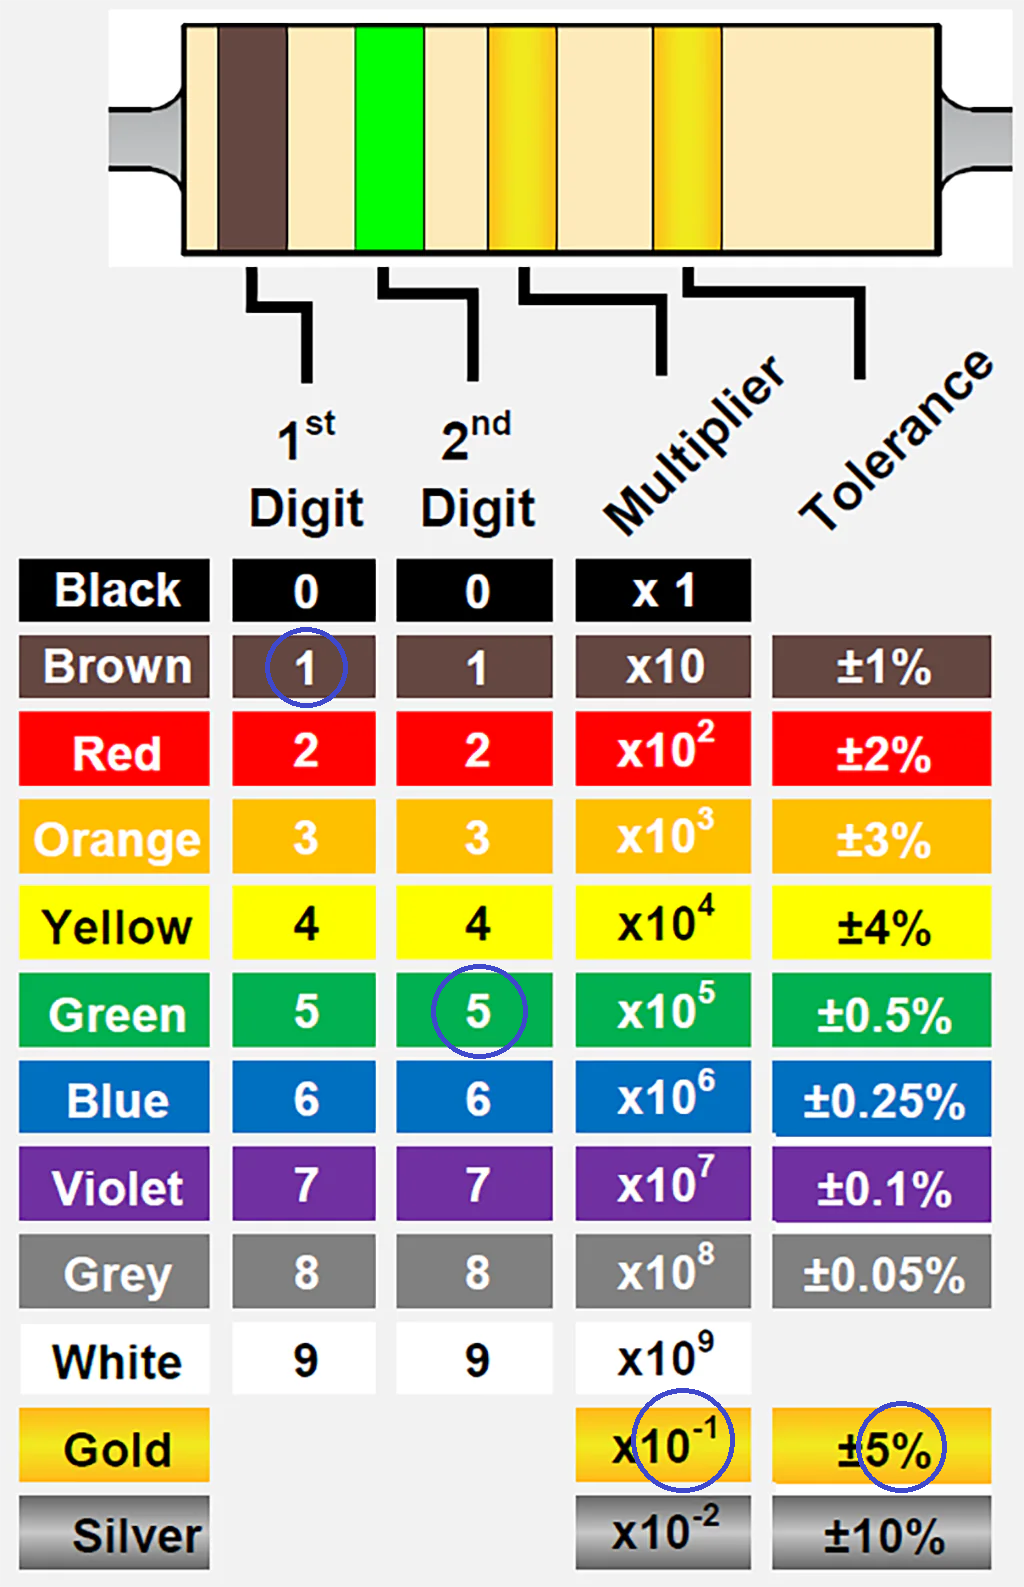
\includegraphics[height=10cm]{Relazione/media/resistoretab.png}
    \caption{Tabella che raffigura il codice dei colori di un resistore}
    \label{fig:resistore}
\end{figure}















\section{Misure di resistenze con multimetro portatile}
\label{sec:mult_port}

\begin{figure}[h]
    \centering
    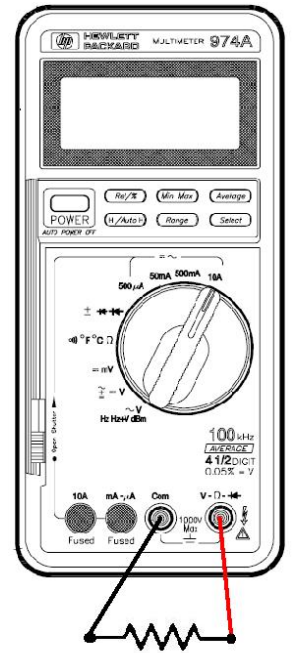
\includegraphics[height=10cm]{Relazione/media/multimetro_port.png}
    \caption{Multimetro utilizzato (Hewlett Packard 974A)}
    \label{fig:multimetro_port}
\end{figure}

Il multimetro HP 974A è dotato di un display a 4 ½ cifre, il quale rappresenta uno strumento con 4 cifre principali e un'ulteriore cifra riservata per indicare il segno e, eventualmente, il valore della cifra più significativa della misurazione. Per calcolare la resistenza con un valore nominale dichiarato dal produttore pari a (1500 ± 7,5) m$\Omega$, abbiamo utilizzato il pulsante "RANGE" per impostare il valore di fondo scala, ovvero il limite superiore che il multimetro può "misurare", a 500 $\Omega$. Dato che lo strumento ha un campo di misura pari a 1/50000 del valore di fondo scala, il passo di quantizzazione, indicato come "Q", è pari a
\begin{equation}
    Q = \frac{V_F_S}{50000} = \frac{500}{50000} = 10 m\Omega
\end{equation}
con un incertezza di quantizzazione pari a: 
\begin{equation}
    U_q = \frac{Q}{2} = 5 m\Omega
\end{equation}

Procediamo con la valutazione dell'incertezza di \textbf{tipo B}, basata sull'utilizzo di informazioni note a priori quali le specifiche metrologiche degli strumenti adoperati. L’incertezza del dispositivo è data da una formula binomia composta da una parte proporzionale alla lettura e da un’altra pari a un numero fisso di LSB, quindi 
 proporzionale alla portata. Le specifiche del costruttore dello strumento, per misure di resistenze, sono le seguenti:

\begin{figure} [h]
    \centering
    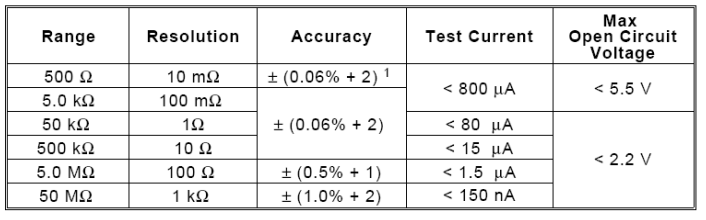
\includegraphics[height=5cm]{Relazione/media/incertezza_port.png}
    \caption{Specifice di incertezza dello strumento utilizzato (Hewlett Packard 974A)}
    \label{fig:Incertezza_multimetro_port}
\end{figure}

Avendo impostato un valore di fondo scala pari a 500 $\Omega$ possiamo notare dalla precedente tabella un’incertezza pari a ±(0,06\% + 2) $\Omega$ , dove il primo termine è proporzionale alla lettura e il secondo alla portata. Si noti che per misure di ampiezza è possibile definire un modello semplificato di uno strumento per misure statiche, del tipo:

\begin{figure} [h]
    \centering
    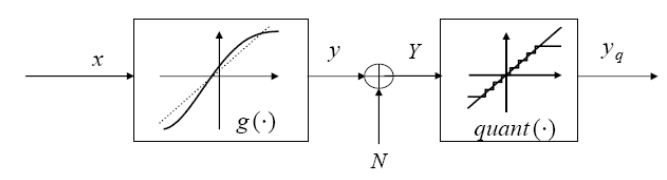
\includegraphics[height=3cm]{Relazione/media/modello_semplificato.png}
    \label{fig:modello}
\end{figure}

Su cui definiamo un errore totale sulla misura del tipo:

\begin{figure} [h]
    \centering
    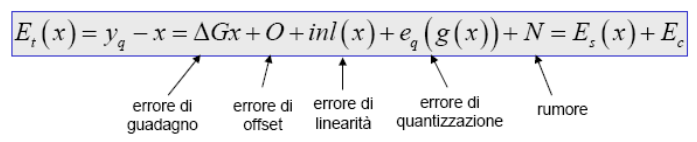
\includegraphics[height=2cm]{Relazione/media/errore_port.png}
    \label{fig:errore port}
\end{figure}

Attraverso una serie di passaggi otteniamo l'incertezza come:
\begin{equation}
    |E_t| \equiv |y_q - x| \equiv | \Delta G_x + O + inl(x) + e_q(g(x)) | \leq 
\end{equation}
(applichiamo una disuguaglianza triangolare)
\begin{equation}
    \leq | \Delta G_x | + | O | + | inl(x) | + | e_q(g(x)) | \leq 
\end{equation}
(applichiamo una disuguaglianza errore-incertezza)
\begin{equation}
    \leq U_G|x| + U_o + U_i_n_l + U_q \cong U_G|y_q| + U_o + U_i_n_l +U_q \equiv U_t_o_t
\end{equation}

Dove, ipotizzando di unire l'incertezza di non linearità integrale nell'incertezza di portata, posso scrivere $U_g$ (incertezza di guadagno), $U_o$ (incertezza di portata dell'offset) e $U_q$ (incertezza di quantizzazione) come: 
\begin{equation}
    \left\{ \begin{array}{rcl}
| \Delta G_x \cdot y_q | \leq U_G |y_q|,    con U_g=0,06\%
\\ | O + inl(x) + e_q(g(x)) | \leq U_o_+_i_n_l_+_q, con U_o_+_i_n_l_+_q=2LSB
\end{array}\right
\end{equation}
Quindi, chiamando Q, passo di quantizzazione e $V_L$ valore letto (supponiamo di usare il primo valore letto nella tabella \label{mult_port}):
\begin{equation}
    U(R) \equiv U_G \cdot V_L + U_o_+_i_n_l_+_q \cdot Q \equiv 0,06\% \cdot 1,62\Omega + 2 \cdot 0,01 \Omega \equiv (0,972 + 20) m\Omega \equiv 0,03 \Omega
\end{equation}
,sapendo che possiamo esprimere la resistenza misurata $R_M$ e il range della resistenza r(R) come:
\begin{equation}
    R_M \equiv(1,62 \pm 0,03) \Omega
\end{equation}
\begin{equation}
    r(R) \equiv [1,59 \Omega \div 1,65 \Omega]
\end{equation}
V\'a notato che l'inclusione dell'errore di non linearit\'a integrale nel secondo termine dell'incertezza fornita dal produttore ( proporzionale alla portata) rende tale termine non solamente un errore di offset puro, ma include anche l'errore di quantizzazione. Pertanto, nel caso di differenze tra misurazioni, non possiamo semplicemente sottrarre l'errore di offset.
Notiamo, usando la resistenza nominale di $(1500 \pm 7,5) m\Omega$ e graficandola con la (2.9) che i due range di valori non sono compatibili.

\begin{figure}[h]
    \centering
    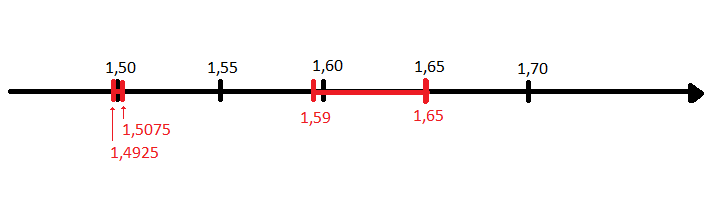
\includegraphics[height=2cm]{Relazione/media/range.png}
    \caption{Differenza dei due range}
    \label{fig:range}
\end{figure}

Effettivamente, la misura eseguita utilizzando il multimetro portatile fornisce una stima non corretta poiché include errori casuali a causa della singola misurazione anziché una media di più valori letti. Inoltre, lo strumento non consente la compensazione degli errori sistematici poiché non dispone di funzioni di calibrazione. Infine, non si è tenuto conto degli errori dovuti alle resistenze di contatto tra i cavi, i puntali e il resistore. Il contributo di tutti questi effetti influisce sul risultato finale della misura.

Se vogliamo quantificare l'accuratezza della misura, assumiamo come valore "vero" della grandezza misurata il valore nominale della resistenza. Facendo questa assunzione, possiamo ottenere una stima dell'errore sistematico come differenza tra il risultato della misura e il valore nominale del componente misurato:
\begin{equation}
    E_S \equiv 1,62 - 1,50 = 0,12\Omega
\end{equation}
L’accuratezza relativa “a” di una misura può essere espressa in funzione di tale errore 
stimato in errore relativo mediante la seguente espressione: 
\begin{equation}
    a \equiv 1 - | \frac{E_S}{R_N_O_M_I_N_A_L_E} | \equiv 92\%
\end{equation}

\newline \newline
\boldsymbol{La} \boldsymbol{nostra} \boldsymbol{prova} \newline

\begin{figure}[h]
    \centering
    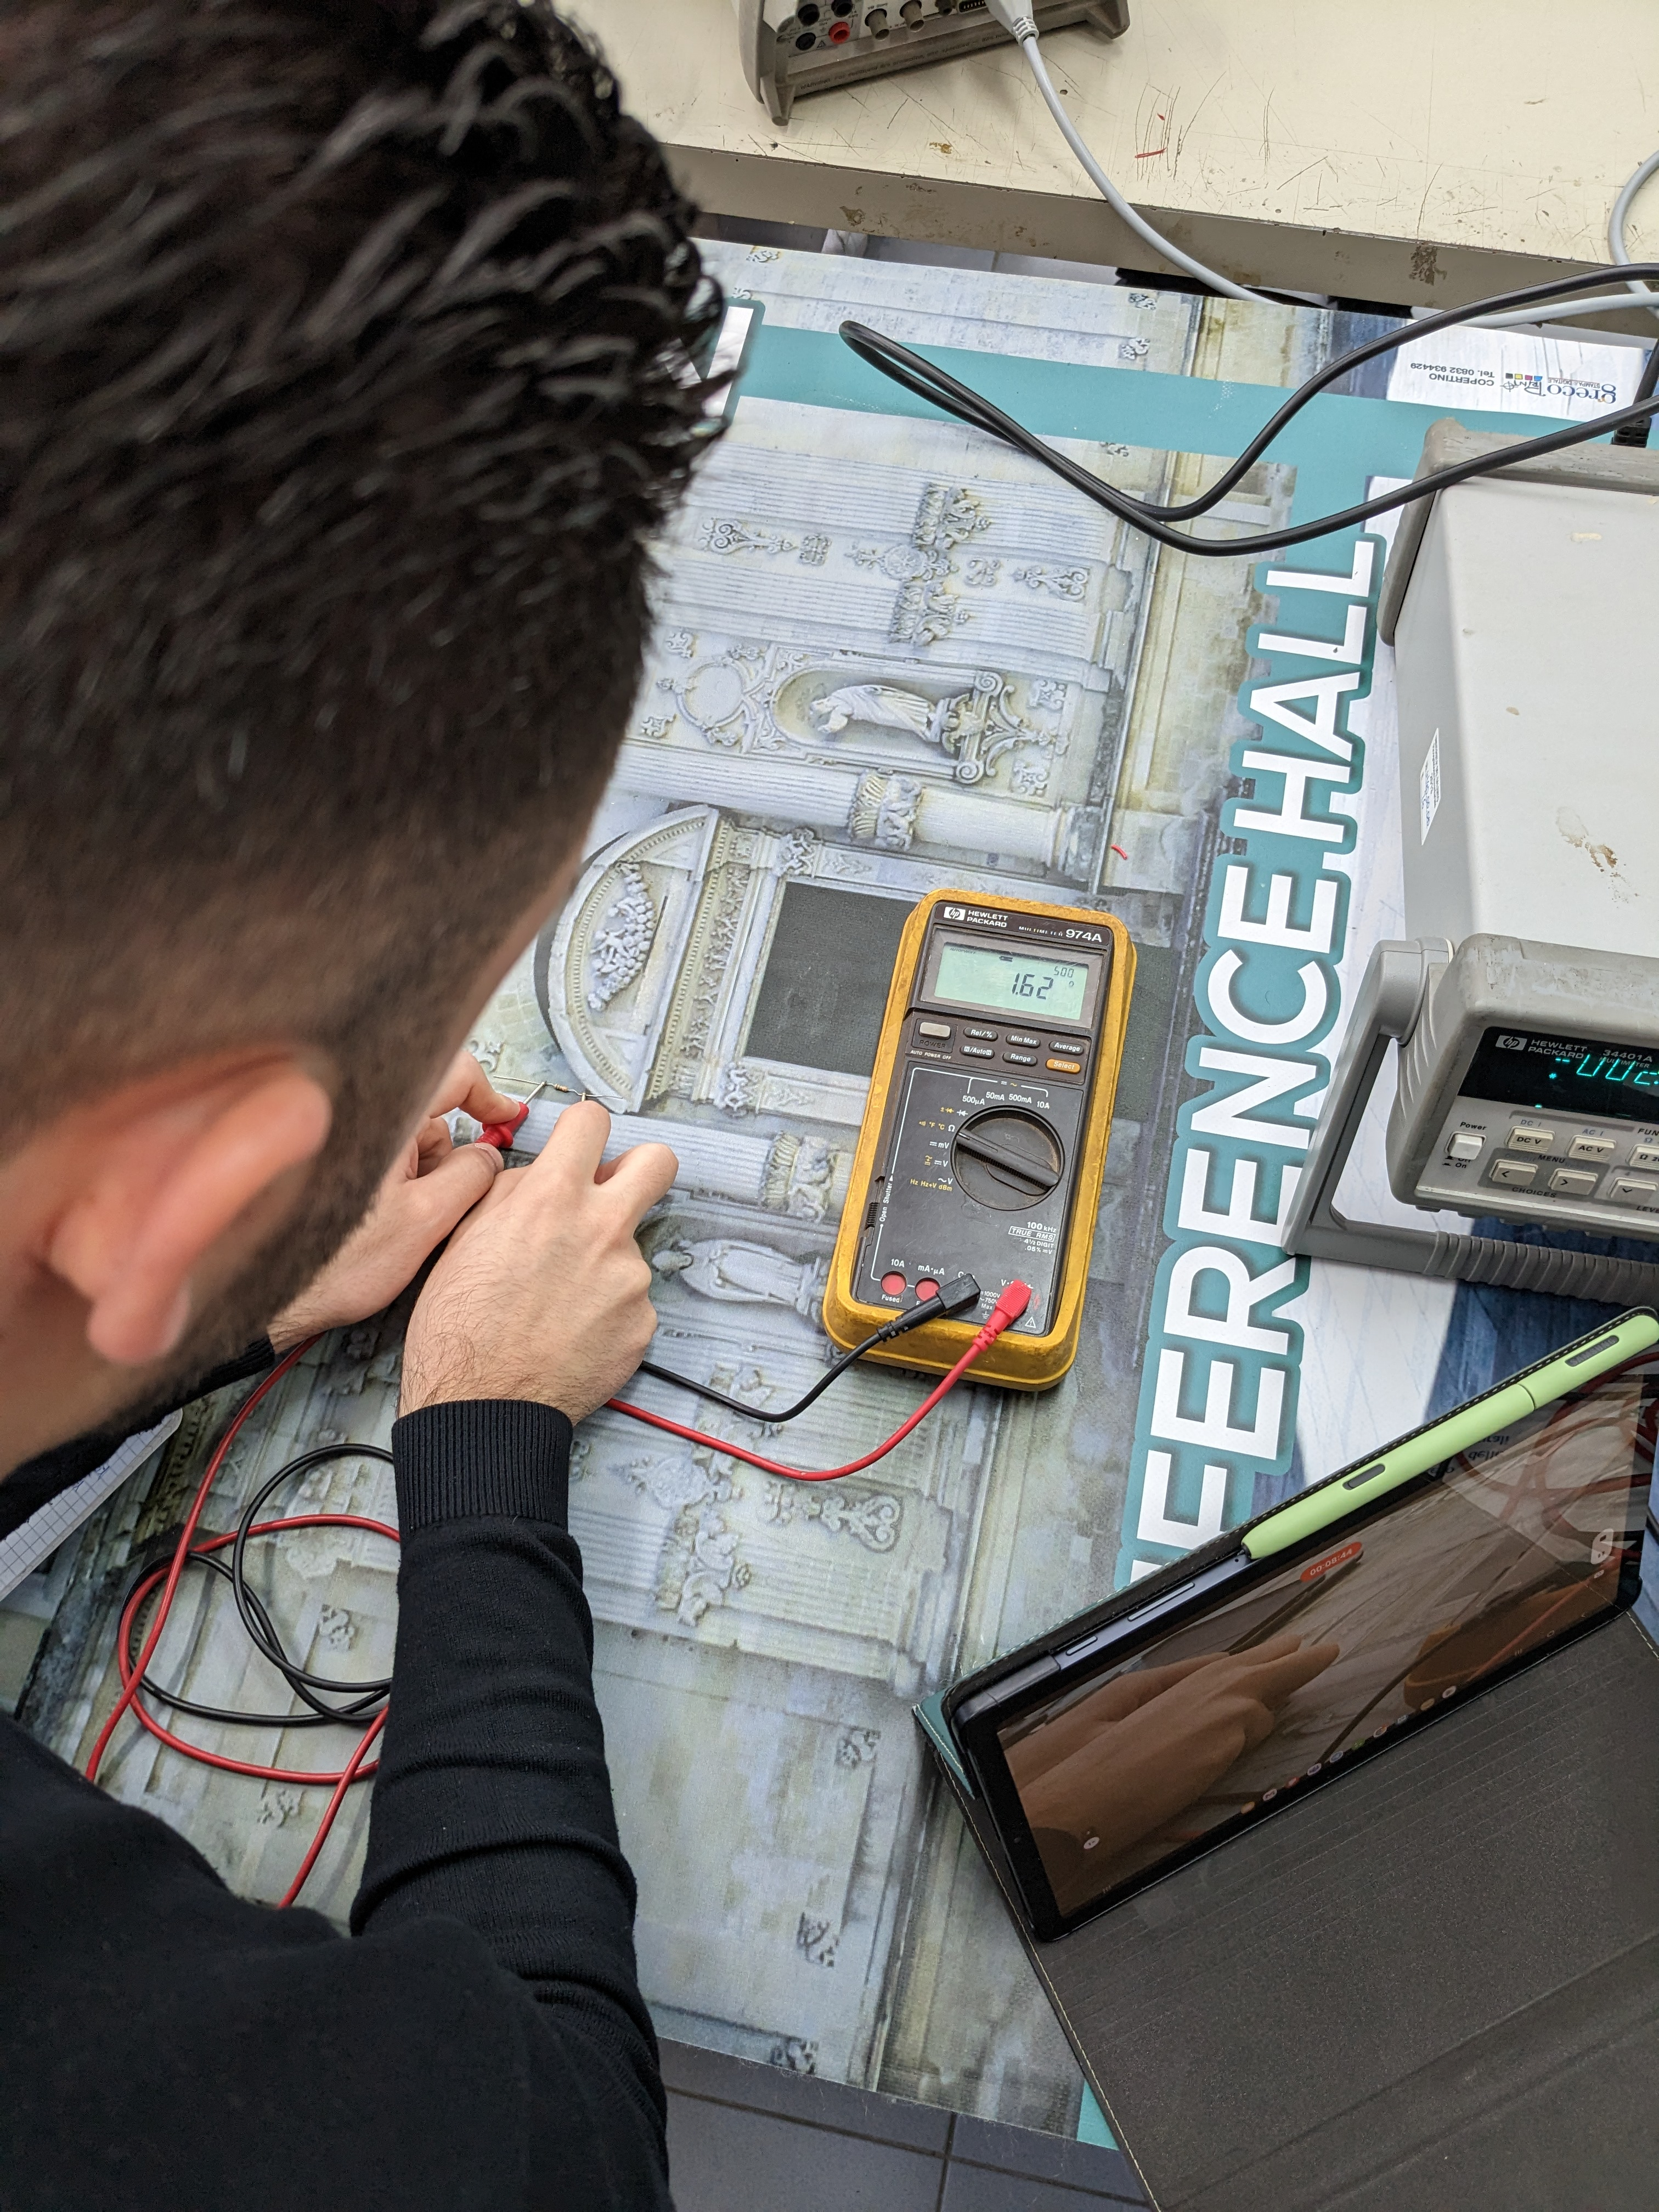
\includegraphics[height=6cm]{Relazione/media/Gameboy_62.jpg}
    \label{fig:mult_port_nostro}
\end{figure}

Quando usiamo il multimetro portatile abbiamo disposto i puntali in maniera pi\'u stabile possibile, applicando una buona pressione per ottenere una misurazione pi\'u fedele possibile,
Abbiamo fatto 10 ripetizioni in modo da ricavare l'incertezza totale, con il contributo valutato di tipo B relativamente alla specifica di strumento utilizzato.

%Per chi vuole inserire tabella usare: https://www.tablesgenerator.com/latex_tables#
%Basta fare ctrl+v sulla tabella di google sheets e andare sul sito , premere File, e fare "Paste table data"

\begin{table}[h]
\centering
\begin{tabular}{|c|c|c|c|}
\hline
\rowcolor[HTML]{6FA8DC} 
Fondo scala 500$\Omega$ & Passo Q ($\Omega$) & Incertezza Uq ($\Omega$) & Incertezza \\ \hline
1,62             & 1,00E-02    & 5,00E-03          & 2,10E-02   \\ \hline
1,61             & 1,00E-02    & 5,00E-03          & 2,10E-02   \\ \hline
1,61             & 1,00E-02    & 5,00E-03          & 2,10E-02   \\ \hline
1,62             & 1,00E-02    & 5,00E-03          & 2,10E-02   \\ \hline
1,60             & 1,00E-02    & 5,00E-03          & 2,10E-02   \\ \hline
1,60             & 1,00E-02    & 5,00E-03          & 2,10E-02   \\ \hline
1,62             & 1,00E-02    & 5,00E-03          & 2,10E-02   \\ \hline
1,61             & 1,00E-02    & 5,00E-03          & 2,10E-02   \\ \hline
1,60             & 1,00E-02    & 5,00E-03          & 2,10E-02   \\ \hline
1,61             & 1,00E-02    & 5,00E-03          & 2,10E-02   \\ \hline
\end{tabular}
\caption{Multimetro portatile 974A}
\label{tab:mult_port}
\end{table}


%---------Multimetro da Banco---------%
\section{Misure di resistenza con multimetro da banco}
\label{sec:mult}


\begin{figure}[h]
    \centering
    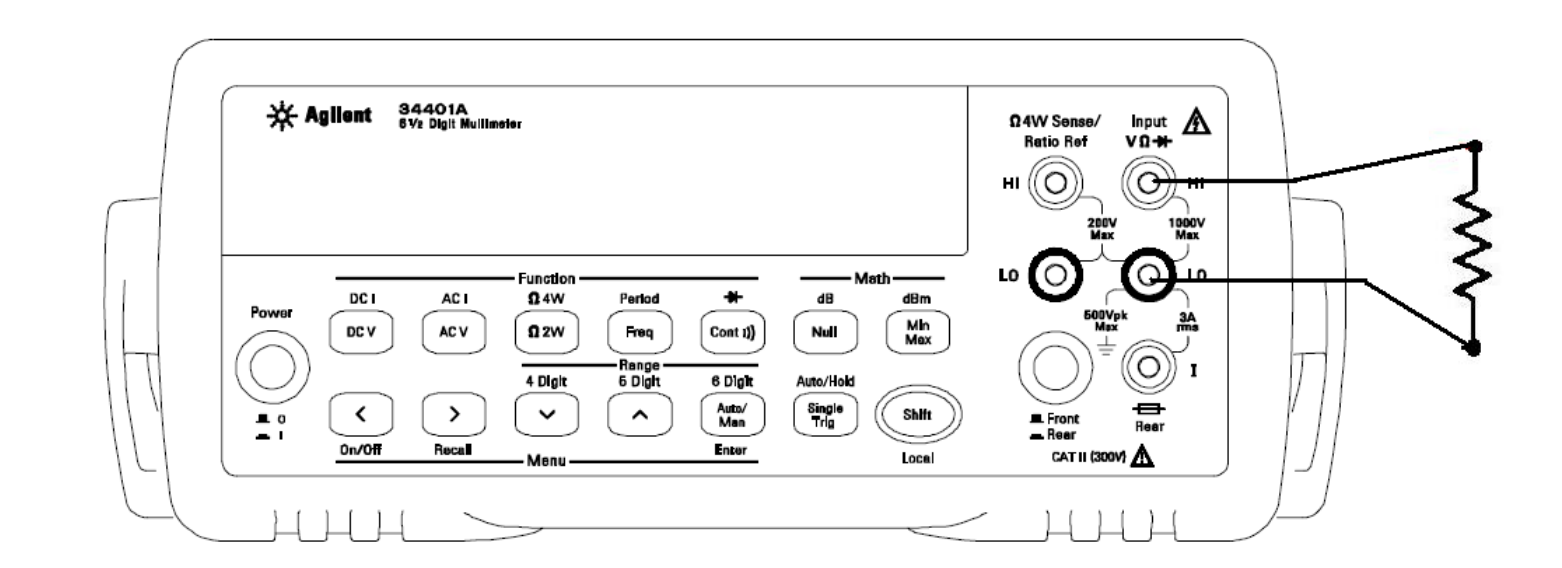
\includegraphics[height=2cm]{Relazione/media/mult_banco.png}
    \caption{Multimetro HP Hewlett Packard 34401A}
    \label{fig:mult_banco}
\end{figure}


Il multimetro HP34401A possiede un display a 6 ½ cifre. 
Per il calcolo della resistenza di valore nominale pari a (1500 ± 7,5) m$\Omega$, impostiamo la portata dello strumento a 100,0000 $\Omega$, lo strumento a 6 ½ cifre ha un campo di misura 
pari a 1/1000000 del valore di fondo scala e quindi il passo di quantizzazione Q sar\'a: 
\begin{equation}
    Q \equiv \frac{V_F_S}{CM} \equiv \frac{10^2}{10^6} = 0,0001 \Omega
\end{equation}
Con l'incertezza di quantizzazione $U_q$ pari a:
\begin{equation}
    U_q \equiv \frac{Q}{CM} \equiv 0,00005 \Omega
\end{equation}

Quando abbiamo lavorato con il multimetro da banco, abbiamo dapprima lavorato in modalità "2 terminali" (attivata premendo la modalità "$\Omega$", e poi "2W" che ci permette di lavorare a due morsetti).

\begin{figure}[h]
    \centering
    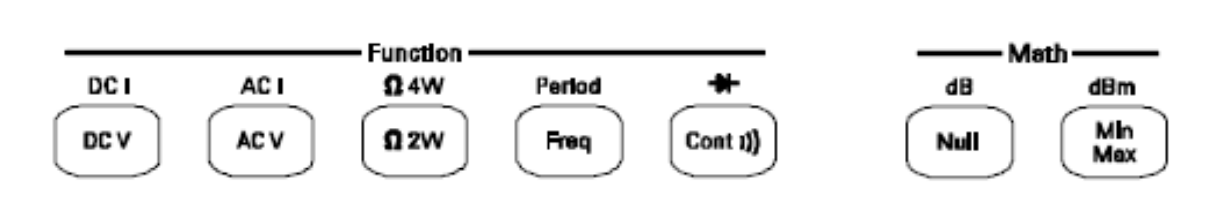
\includegraphics[height=2cm]{Relazione/media/mult_banco_zoom.png}
    \caption{Zoom sui tasti premuti}
    \label{fig:mult_banco_zoom}
\end{figure}

Come prima operazione abbiamo cortocircuitato i morsetti, premendo il tasto null, in modo che il valore di resistenza interna del conduttore dei cavi venga preso in considerazione permettendoci di tarare lo strumento, mostrando una misurazione prossima a zero (nel nostro caso abbiamo visualizzato a display, impostato a 6 cifre e mezzo, il valore 0,000134).


\begin{figure}[h]
    \centering
    \includegraphics[height=5cm]{Relazione/media/2Morsetti_432.jpg}
    \label{fig:2morsetti}
\end{figure}

\'E importante notare che se la resistenza dei cavi è comparabile o superiore alla resistenza che si desidera misurare, il risultato della misura potrebbe essere influenzato significativamente dal contributo della resistenza dei cavi, dunque per ridurre gli errori sistematici:
\begin{equation}
    Risultato = Valore letto - Valore NULL
\end{equation}

\begin{figure}[h]
    \centering
    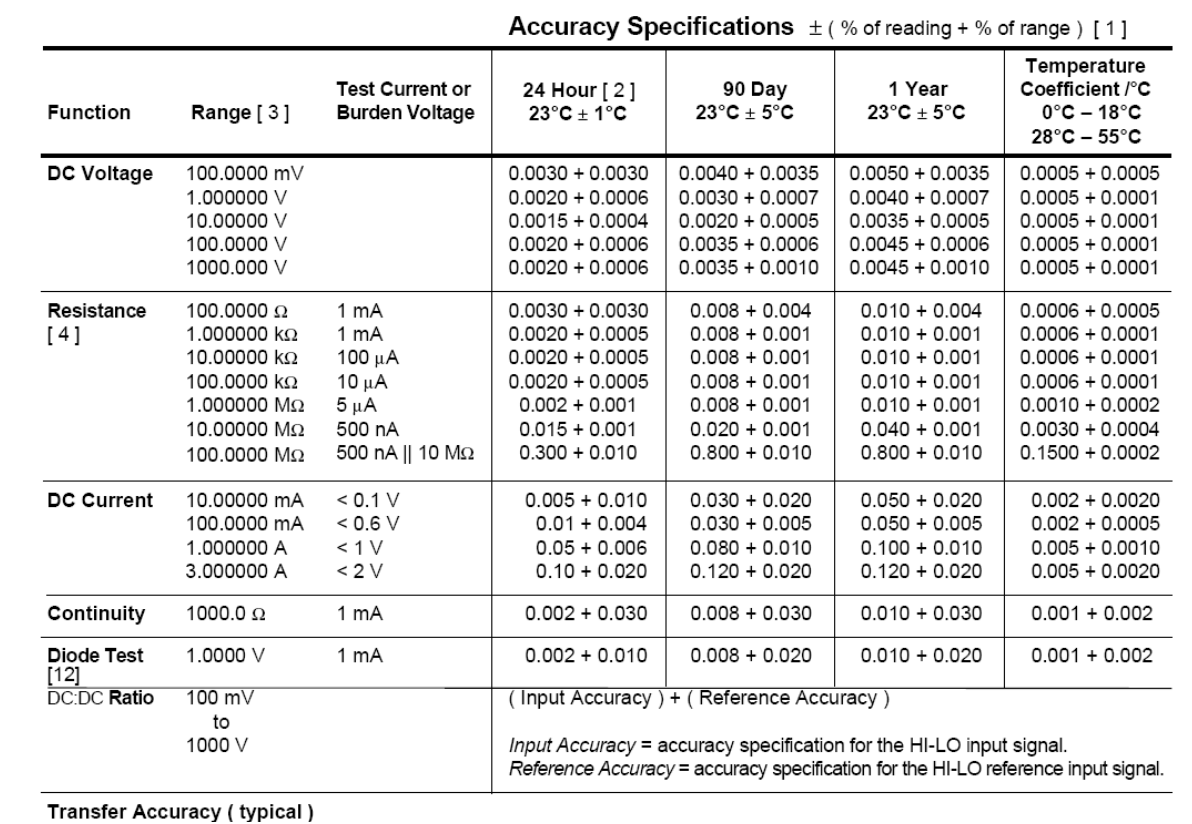
\includegraphics[height=5cm]{Relazione/media/tabella_mult_banco.png}
    \label{fig:tab_mult_banco}
\end{figure}

Avendo impostato un valore di fondo scala pari a 100,0000 $\Omega$, in un ambiente con una temperatura pari a (23 $\pm$ 5)°C, facciamo riferimento all'incertezza $\pm$(0,010 $\% \pm 0,004 \%$), con il primo termine proporzionale alla lettura e il secondo proporzionale alla portata.
Ragionando come prima, ipotizzando di unire l'incertezza di non linearità integrale nell'incertezza di portata, posso scrivere $U_g$ (incertezza di guadagno), $U_o$ (incertezza di portata dell'offset) e $U_q$ (incertezza di quantizzazione) come: 
\begin{equation}
    \left\{ \begin{array}{rcl}
| \Delta G \cdot y_q | \leq U_G |y_q|,    con U_g=0,01\%
\\ | O + inl(x) + e_q(g(x)) | \leq U_o_+_i_n_l_+_q, con U_o_+_i_n_l_+_q=0,004\%
\end{array}\right
\end{equation}
Quindi, chiamando P, portata e $V_L$ valore letto (supponiamo di usare il primo valore letto nella tabella \label{mult_port}):
\begin{equation}
    U(R) \equiv U_G \cdot V_L + U_o_+_i_n_l_+_q \cdot P \equiv 0,01\% \cdot 1,648\Omega + 0,004 \% \cdot 100 \Omega \equiv 0,004 \Omega (arrotondato per difetto)
\end{equation}

\begin{table}[h] %la h serve per metterla esattamente dove la si sta mettendo nel file in Latex
\centering
\resizebox{\textwidth}{!}{
\begin{tabular}{|c|c|c|c|c|c|cl|}
\hline
\rowcolor[HTML]{CFE2F3} 
Misure ($\Omega$) & Valore di NULL - Cortocircuito (V) & Risultato & Fondo scala ($\Omega$) & Passo Q ($\Omega$) & Incertezza Uq ($\Omega$) & \multicolumn{2}{c|}{\cellcolor[HTML]{CFE2F3}Incertezza} \\ \hline
1,648 & 0,133 & 1,515 & 100 & 0,0001 & 0,00005 & \multicolumn{2}{c|}{0,0041515} \\ \hline
1,614 & 0,133 & 1,481 & 100 & 0,0001 & 0,00005 & \multicolumn{2}{c|}{0,0041481} \\ \hline
1,627 & 0,133 & 1,494 & 100 & 0,0001 & 0,00005 & \multicolumn{2}{c|}{0,0041494} \\ \hline
1,614 & 0,133 & 1,481 & 100 & 0,0001 & 0,00005 & \multicolumn{2}{c|}{0,0041481} \\ \hline
1,432 & 0,133 & 1,299 & 100 & 0,0001 & 0,00005 & \multicolumn{2}{c|}{0,0041299} \\ \hline
1,466 & 0,133 & 1,333 & 100 & 0,0001 & 0,00005 & \multicolumn{2}{c|}{0,0041333} \\ \hline
1,441 & 0,133 & 1,308 & 100 & 0,0001 & 0,00005 & \multicolumn{2}{c|}{0,0041308} \\ \hline
1,468 & 0,133 & 1,335 & 100 & 0,0001 & 0,00005 & \multicolumn{2}{c|}{0,0041335} \\ \hline
1,475 & 0,133 & 1,342 & 100 & 0,0001 & 0,00005 & \multicolumn{2}{c|}{0,0041342} \\ \hline
1,493 & 0,133 & 1,36  & 100 & 0,0001 & 0,00005 & \multicolumn{2}{c|}{0,004136}  \\ \hline
\end{tabular}
}
\caption{Multimetro 34401A (6$\sfrac{1}{2}$ cifre), 2 Morsetti}
\label{tab:mult_2w}
\end{table}



\newline \newline \newline
 Sapendo che la resistenza misurata col multimetro è 1,648 $\Omega$, il risultato della misura si esprime come R=(+1,648 $\pm$ 0,005)$\Omega$, abbiamo operato anche con un sistema a quattro morsetti(metodo Kelvin)


\begin{figure}[h]
    \centering
    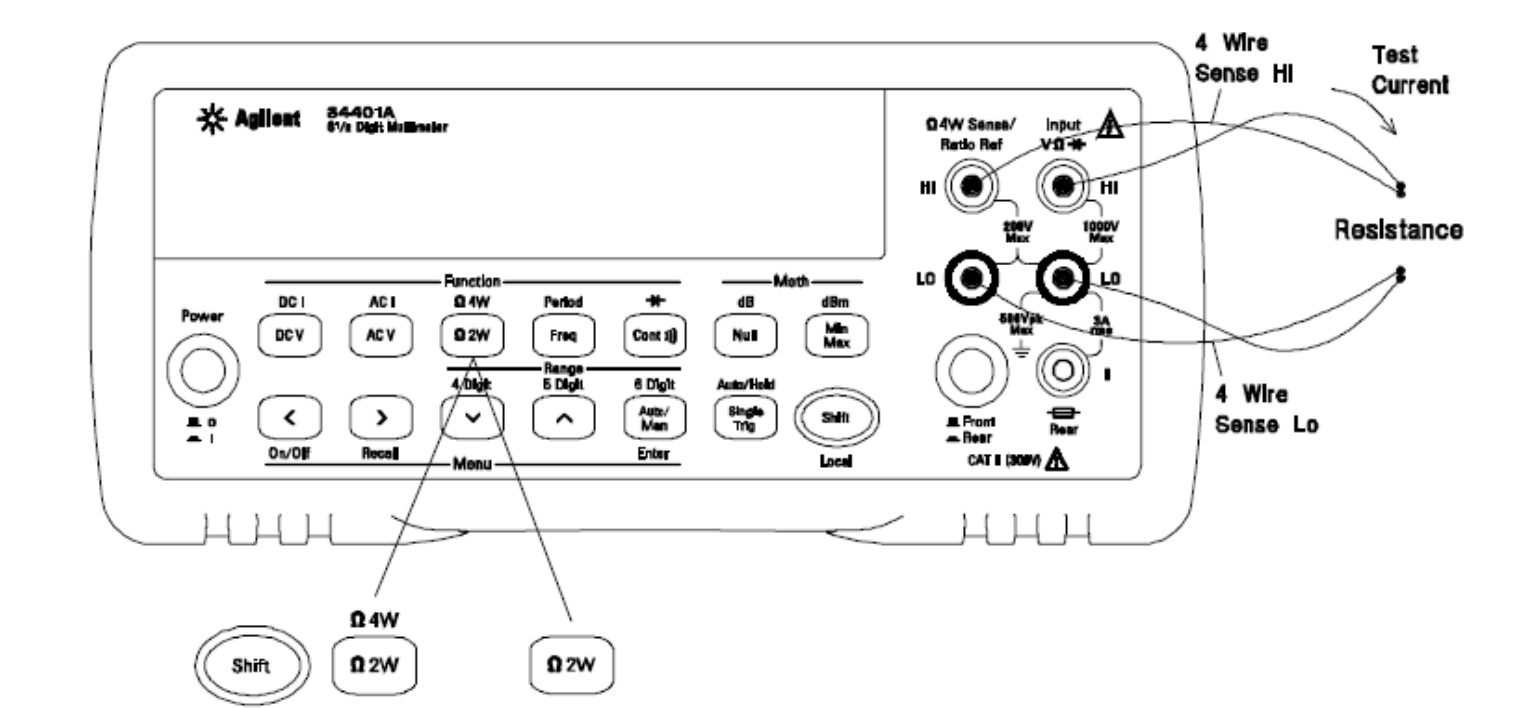
\includegraphics[height=5cm]{Relazione/media/quattro_morsetti.png}
    \caption{Metodo Kelvin a 4 morsetti}
    \label{fig:quattro morsetti}
\end{figure}





Successivamente, sempre con lo stesso multimetro da banco, abbiamo lavorato in modalità "4 terminali" (attivata sempre premendo la modalità "$\Omega$", e poi successivamente "4W" per lavorare a quattro morsetti).

\begin{figure}[h]
    \centering
    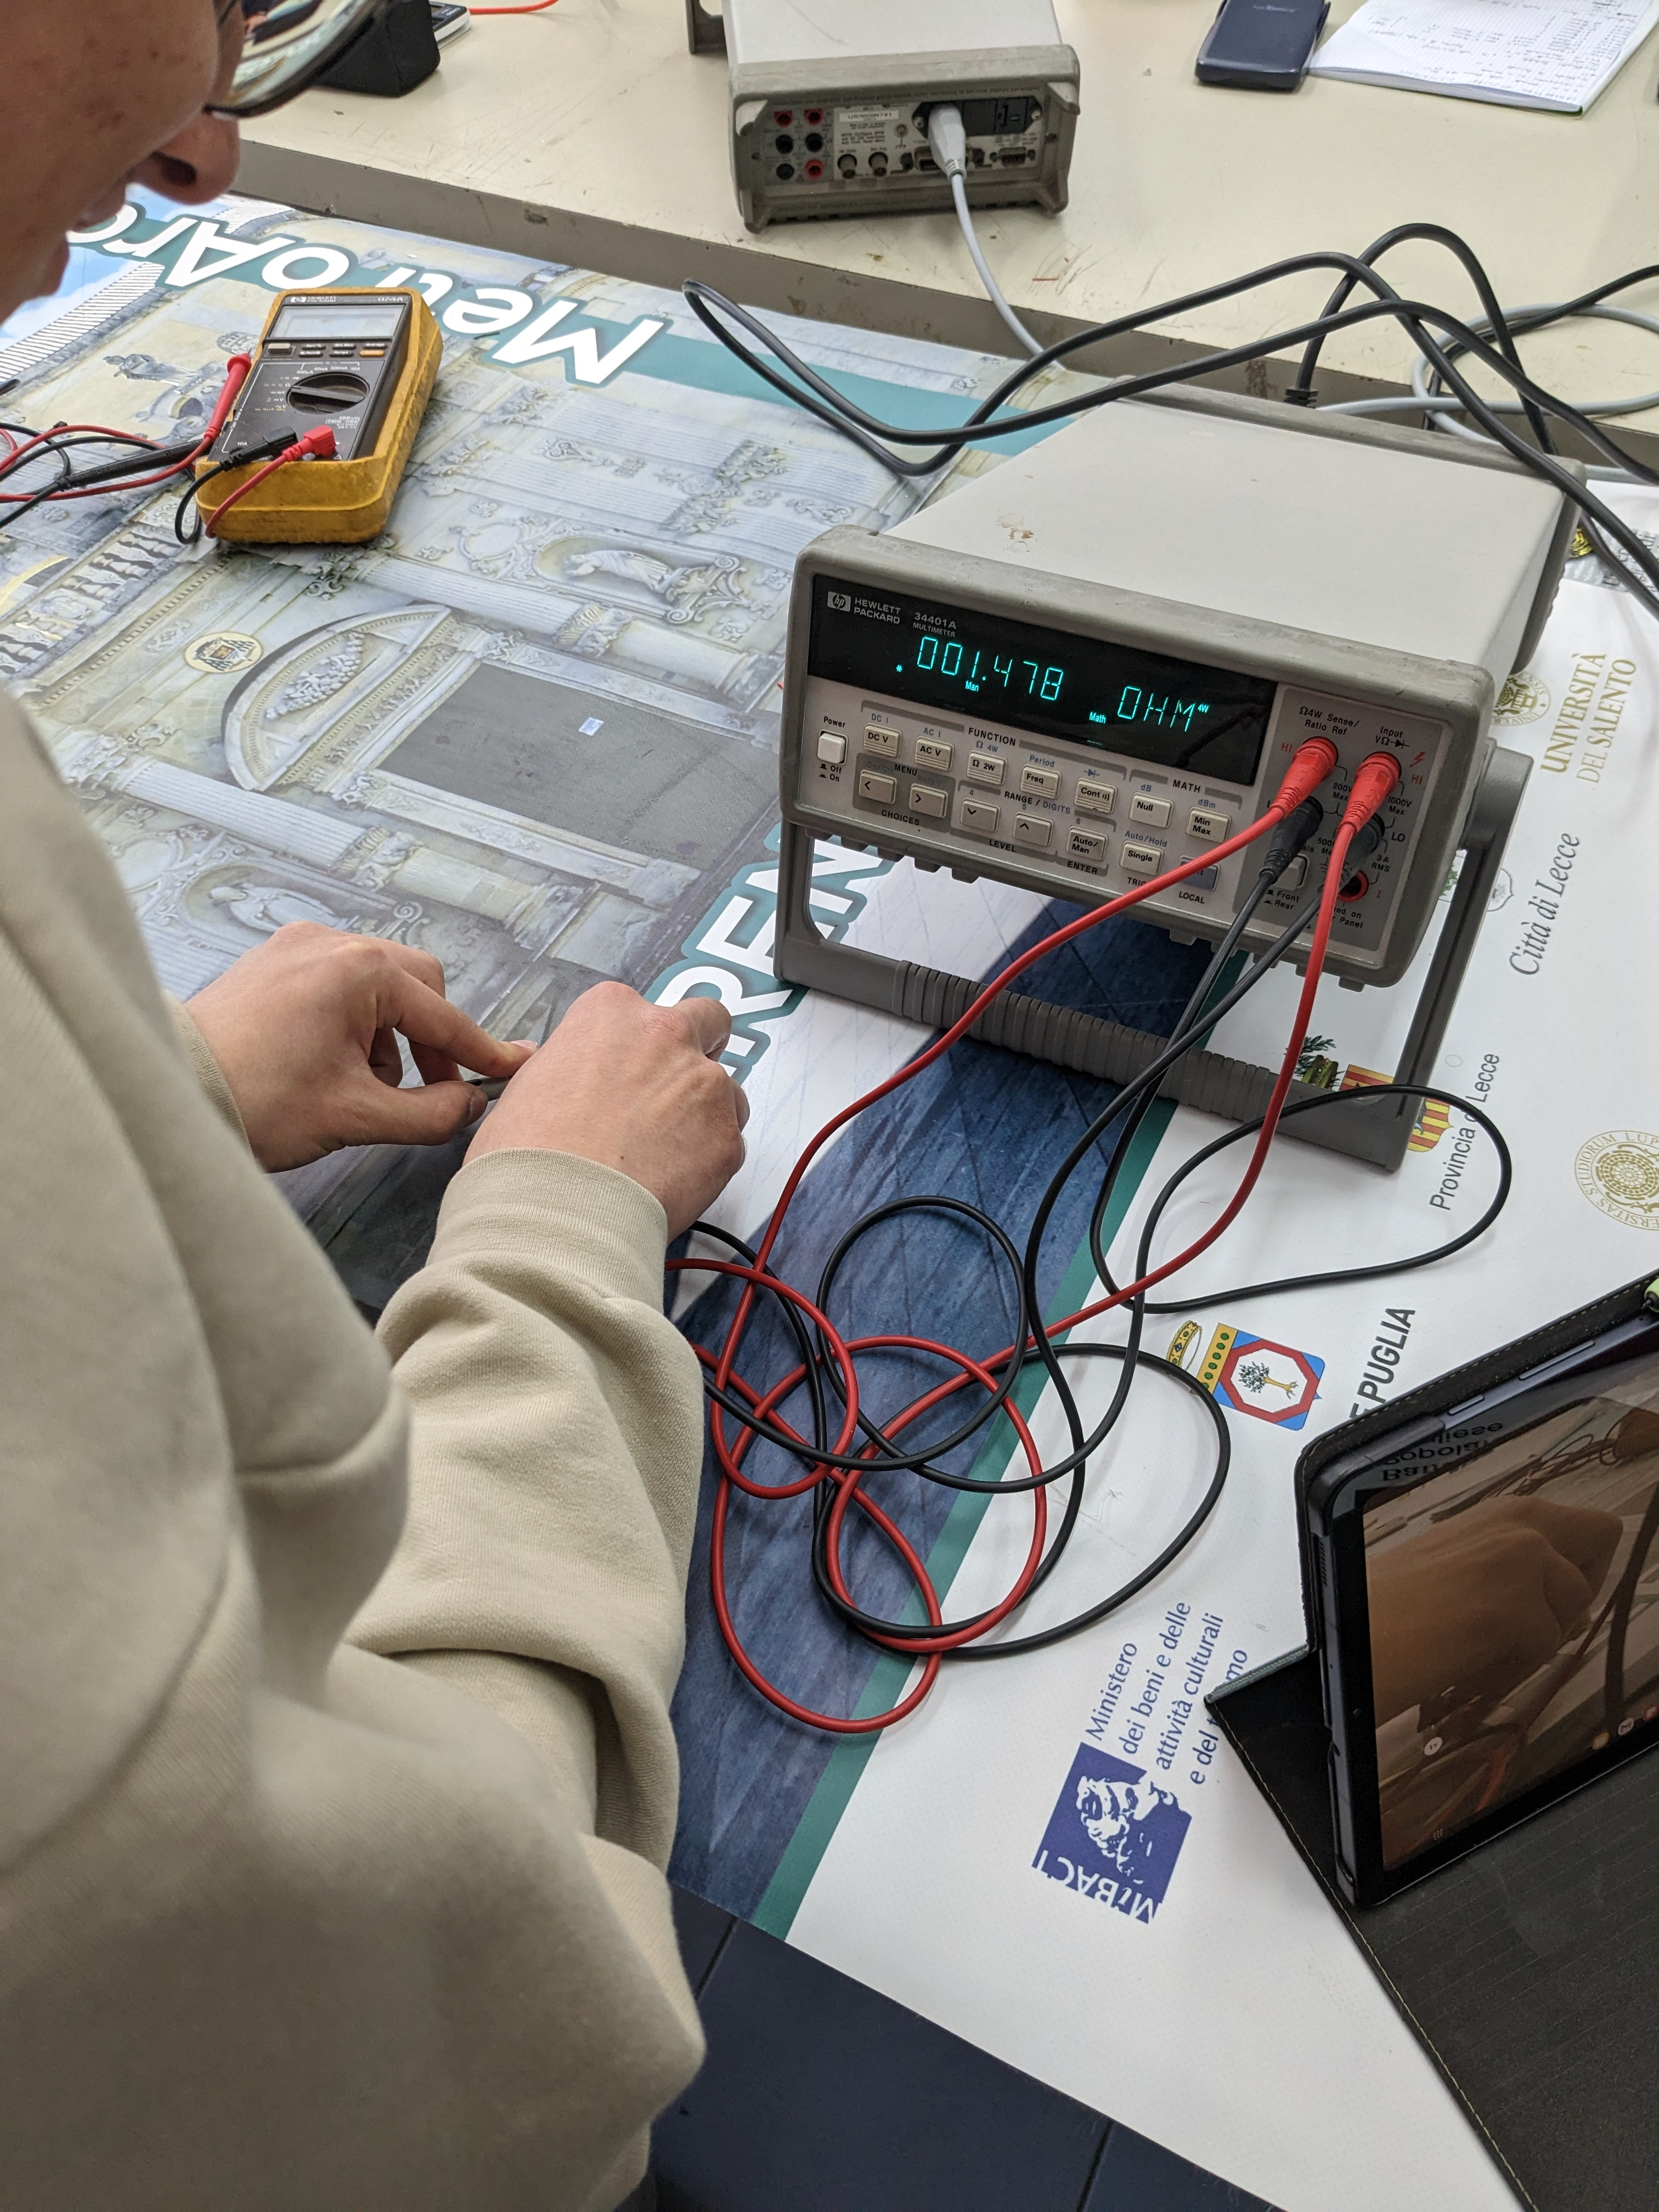
\includegraphics[height=5cm]{Relazione/media/4Morsetti_472.jpg}
    \label{fig:4morsetti}
\end{figure}
Anche in questo caso abbiamo nuovamente cortocircuitato i morsetti, premendo nuovamente il tasto null per tarare lo strumento e riavere un valore associato al cortocircuito pi\'u prossimo allo zero possibile in presenza del cortocircuito (nel nostro caso 0,004).


Attraverso la prima coppia di morsetti (Hi, Lo), lo strumento inietta la corrente nota come "$I_0$" nella resistenza. Questa corrente attraversa le boccole (Hi, Lo) dove si incontra con la resistenza di contatto, che può falsare la misura standard a due fili (impostando $\Omega$2W sul pannello frontale del multimetro).

Per evitare questo problema, tramite l'altra coppia di morsetti di sensing (Hi, Lo), viene prelevata la tensione su due punti più vicini al resistore. Utilizzando questa configurazione (impostando $\Omega$4W sul pannello frontale del multimetro), le cadute di tensione sulle resistenze di contatto presenti sulle boccole che portano la corrente al resistore in prova possono essere escluse dalla tensione da misurare, garantendo una misurazione più accurata.

Si effettua l'operazione di NULL in modo analogo al caso precedente, misurando un valore di resistenza pari a R = 1,478 Ω. Dalla teoria, questo valore dovrebbe essere più accurato rispetto al caso del multimetro a due morsetti. Utilizzando il modello precedente per il calcolo dell'incertezza, otteniamo:
\begin{equation}
    \left\{ \begin{array}{rcl}
| \Delta G \cdot y_q | \leq U_G |y_q|,    con U_g=0,01\%
\\ | O + inl(x) + e_q(g(x)) | \leq U_o_+_i_n_l_+_q, con U_o_+_i_n_l_+_q=0,004\%
\end{array}\right
\end{equation}
Quindi, chiamando P, portata e $V_L$ valore letto (supponiamo di usare il primo valore letto nella tabella \label{mult_port}):
\begin{equation}
    U(R) \equiv U_G \cdot V_L + U_o_+_i_n_l_+_q \cdot P \equiv 0,01\% \cdot 1,478\Omega + 0,004 \% \cdot 100 \Omega \equiv 0,004 \Omega 
\end{equation}
(dove il risultato è stato arrotondato per difetto)
Notiamo che l’incertezza in questo caso non è cambiata, con R=(+1,478 $\pm$ 0,005)$\Omega$



\begin{table}[h]
\centering
\resizebox{\textwidth}{!}{%
\begin{tabular}{|c|c|c|c|c|c|cl|}
\hline
\rowcolor[HTML]{CFE2F3} 
\multicolumn{1}{|l|}{\cellcolor[HTML]{CFE2F3}Misure ($\Omega$)} &
  \multicolumn{1}{l|}{\cellcolor[HTML]{CFE2F3}Valore di NULL (V) ??} &
  \multicolumn{1}{l|}{\cellcolor[HTML]{CFE2F3}Risultato} &
  \multicolumn{1}{l|}{\cellcolor[HTML]{CFE2F3}Fondo scala ($\Omega$)} &
  \multicolumn{1}{l|}{\cellcolor[HTML]{CFE2F3}Passo Q ($\Omega$)} &
  \multicolumn{1}{l|}{\cellcolor[HTML]{CFE2F3}Incertezza Uq ($\Omega$)} &
  \multicolumn{2}{l|}{\cellcolor[HTML]{CFE2F3}Incertezza} \\ \hline
1,478 & 0,004 & 1,474 & 100 & 0,0001 & 0,00005 & \multicolumn{2}{c|}{0,0041474} \\ \hline
1,478 & 0,004 & 1,474 & 100 & 0,0001 & 0,00005 & \multicolumn{2}{c|}{0,0041474} \\ \hline
1,478 & 0,004 & 1,474 & 100 & 0,0001 & 0,00005 & \multicolumn{2}{c|}{0,0041474} \\ \hline
1,478 & 0,004 & 1,474 & 100 & 0,0001 & 0,00005 & \multicolumn{2}{c|}{0,0041474} \\ \hline
1,478 & 0,004 & 1,474 & 100 & 0,0001 & 0,00005 & \multicolumn{2}{c|}{0,0041474} \\ \hline
1,478 & 0,004 & 1,474 & 100 & 0,0001 & 0,00005 & \multicolumn{2}{c|}{0,0041474} \\ \hline
1,478 & 0,004 & 1,474 & 100 & 0,0001 & 0,00005 & \multicolumn{2}{c|}{0,0041474} \\ \hline
1,478 & 0,004 & 1,474 & 100 & 0,0001 & 0,00005 & \multicolumn{2}{c|}{0,0041474} \\ \hline
1,478 & 0,004 & 1,474 & 100 & 0,0001 & 0,00005 & \multicolumn{2}{c|}{0,0041474} \\ \hline
1,478 & 0,004 & 1,474 & 100 & 0,0001 & 0,00005 & \multicolumn{2}{c|}{0,0041474} \\ \hline
\end{tabular}%
}
\caption{Multimetro 34401A (6$\sfrac{1}{2}$ cifre), 4 Morsetti}
\label{tab:mult_4w}
\end{table}




\newline \newline \newline

Osserviamo questa volta che utilizzando il multimetro da banco a 6 ½ cifre si ottiene una stima più precisa del valore misurato rispetto all'utilizzo del multimetro portatile descritto precedentemente. Questi miglioramenti possono essere attribuiti alla capacità dello strumento da banco di ridurre gli errori sistematici mediante l'implementazione di funzioni adeguate.

Il multimetro da banco a 6 ½ cifre offre una maggiore precisione grazie alla sua elevata risoluzione e alla possibilità di compensare gli errori sistematici tramite funzioni avanzate di calibrazione e correzione. Ciò consente di ottenere misurazioni più accurate e affidabili, riducendo l'effetto degli errori di offset, delle non linearità e di altri fattori che potrebbero influenzare la precisione della misura.

Inoltre, lo strumento da banco può offrire un controllo più preciso delle condizioni operative, come la compensazione della resistenza dei cavi o la selezione della modalità di misura più adatta alle specifiche dell'applicazione. Ciò contribuisce ulteriormente a migliorare l'accuratezza complessiva della misurazione.

In conclusione, usando una resistenza con valore nominale di (1500 ± 7,5) m$\Omega$, con il multimetro da banco otteniamo una stima pari a R=(+1,648 $\pm$ 0,005)$\Omega$ per la misurazione a due morsetti, mente otteniamo una stima pari a R=(+1,478 $\pm$ 0,005)$\Omega$ per la misurazione a 4 morsetti.

\begin{figure}[h]
    \centering
    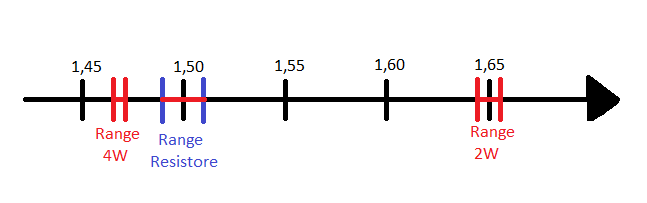
\includegraphics[height=3cm]{Relazione/media/banco_misure.png}
    \label{fig:range}
\end{figure}

eeeeeeeeeeeeeeeeeeeeeeeeeeeeeeeeeeeeeeeeeee doveva uscire che i 4w stava dentro il range del resistore, non so se dovremmo commentare o no la cosaaaaaaaaaaaaaaaaaaaaaaaaaaaaaaaaaaaaa
\newline
Volendo quantificare gli errori sistematici:
\begin{equation}
    E_S_(_2_W_) \equiv 1,648 - 1,500 = 0,148 \Omega
\end{equation}
\begin{equation}
    | E_S_(_4_W_) | \equiv | 1,478 - 1,500  |= 0,022 \Omega
\end{equation}
che portano alle seguenti accuratezze: 
\begin{equation}
    a_(_2_W_) \equiv 1 - | \frac{E_S_(_2_W_)}{R_N_O_M_I_N_A_L_E} | \equiv 91\%
\end{equation}
\begin{equation}
    a_(_4_W_) \equiv 1 - | \frac{E_S_(_4_W_)}{R_N_O_M_I_N_A_L_E} | \equiv 91\%
\end{equation}

AIUTOOOOOOOOOOOOOOO dovrebbero essere percentuali pi§ alte del multimetro da banco














%----------LCR-----------%
\section{Misure con LCR-Meter}
\label{sec:lcr}

COSè IL LCR METER (INTRODUZIONEEEEEEEEEEEEEEEEEEEEEEEEEEEEEEEEEEEEEEEEEEEEEEEEEEEEEEEEEEEEEEEEEEEEEEEEEEEEEEEEEEEEEEEEEE) + FOTOOOOOOOOOOOOOOOOOOOOO


\subsection{Impedenze}
\label{sub:z}

Tramite l'LCR-Meter abbiamo svolto l'ultima parte della nostra prima esperienza.
Innanzitutto abbiamo calibrato lo strumento per compensare gli errori sistematici introdotti dallo strumento stesso, dando come riferimento due carichi noti (il circuito virtualmente chiuso e aperto), premendo sul tassto blu dello strumento e aspettando la dicitura "short correction complete".
Per fare la prova, abbiamo avuto la possibilità di impostare vari valori di frequenza a partire da 100Hz, abbiamo impostato un tempo di misura medio ??? e impostato il modello capacità ideale con collegamento parallelo (premendo in successione i tasti CP-D e CP-RP).
Partiamo con i 100Hz, e misuriamo la resistenza (R) e reattanza (X, nel nostro caso leggermente negativà perché prevale l'effetto induttivo). Abbiamo fatto così per ogni valore della frequenza presente nella seguente tabella.  


\begin{table}[ht]
\centering
\resizebox{\textwidth}{!}{%
\begin{tabular}{|c|c|c|}
\hline
\rowcolor[HTML]{CFE2F3} 
\textit{Frequenza {[}Hz{]}} & R {[}$\Omega${]} & X {[}m$\Omega${]} \\ \hline
100Hz                       & 1,4630    & -0,04      \\ \hline
120Hz                       & 1,4628    & -0,05      \\ \hline
1kHz                        & 1,4625    & -0,52      \\ \hline
10kHz                       & 1,4622    & -5,12      \\ \hline
100kHz                      & 1,4635    & -51,50     \\ \hline
\end{tabular}%
}
\caption{LCR, misura Impedenza, Tempo di misura: Long}
\label{tab:lcr_z}
\end{table}

\begin{table}
\centering
\resizebox{\textwidth}{!}{%
\begin{tabular}{|c|c|c|c|c|c|c|c|}
\hline
\rowcolor[HTML]{CFE2F3} 
A      & B      & C & D {[}$\Omega${]} & E {[}$\Omega${]} & Zs {[}$\Omega${]} & Zx {[}$\Omega${]} & Uz (Ae) \\ \hline
0,005  & 0,0009 & 1 & 0,01      & 2,80E+08  & 1          & 1,4630     & 0,0125  \\ \hline
0,005  & 0,0009 & 1 & 0,01      & 2,80E+08  & 1          & 1,4628     & 0,0125  \\ \hline
0,004  & 0,0003 & 1 & 0,0165    & 2,80E+07  & 1          & 1,4625     & 0,0155  \\ \hline
0,004  & 0,0003 & 1 & 0,075     & 2,80E+06  & 1          & 1,4622     & 0,0555  \\ \hline
0,0097 & 0,0011 & 1 & 0,75      & 2,80E+05  & 1          & 1,4635     & 0,5229  \\ \hline
\end{tabular}%
}
\caption{Tabella di incertezza fornita dal costruttore, con Uz l'incertezza}
\label{tab:lcr_z_sheet}
\end{table}



%-------------Capacità----------- NON CAPISCO PERCHé LA METTE PRIMA DELLE TABELLE #*+ç-*°à°°àààAAAAAAAAAAAAAAAAAAAAAAAAAAAAAAAAAAAAAAAAAAAAAA%
\subsection{Capacità}
\label{sub:c}
Come ultima parte della prova abbiamo misurato la capacità del condensatore.
Premiamo in successione "CP" (capacità), "RP" (resistenza parallela) e poi "D" (per il valore della tangente dell'angolo di perdita). Questa procedura è stata ripetuta per tutti i valori di frequenza (partendo da 100kHz, arrivando fino ai 100Hz).


\begin{table}[ht]
\centering
\caption{LCR, misura della capacità}
\label{tab:lcr_c}
\end{table}





    
    %\hypersetup{hidelinks}
    %\chapter{Misure di resistenza con multimetro da banco}
\label{chap:mult}

    
    %\hypersetup{hidelinks}
    %\chapter{Misure di impedenze con LCR-Meter}
\label{chap:lcr}
    
    
    % blank page
    \newpage
    \mbox{}
    \thispagestyle{empty}
\end{document}
